\documentclass[a4paper]{article}
\usepackage{amsfonts, amsmath, amssymb, physics}
\usepackage[utf8]{inputenc}
\usepackage[english]{babel}
\usepackage{indentfirst}
\usepackage[backend=biber, citestyle=nature]{biblatex}
\usepackage[nottoc]{tocbibind}
\usepackage{halloweenmath}
\usepackage{calligra}
\usepackage{esint}
\usepackage{graphicx}
\graphicspath{{./images/}}

%%%%%%%%%%%%%%%%%%%%% PREAMBLE %%%%%%%%%%%%%%%%%%%%%%%%
\setlength{\parindent}{2em}
\setlength{\parskip}{0em}

\newcommand{\dmr}[1]{\, \mathrm{d}#1} %command for the straight d (hehe)
\newcommand{\intt}[2]{\int_{#1}^{#2}} %easy intergral command


\newtheorem{definition}{Definition}[section]
\newtheorem{theorem}{Theorem}[section]
\newtheorem{remark}{Remark}[subsubsection]

\numberwithin{equation}{subsection}

\addbibresource{ref.bib}


\DeclareMathAlphabet{\mathcalligra}{T1}{calligra}{m}{n}
\DeclareFontShape{T1}{calligra}{m}{n}{<->s*[2.3]callig15}{}
\newcommand{\curly}[1]{\ensuremath{\mathcalligra{#1}}}
%%%%%%%%%%%%%%%%%%%%%%%%%%%%%%%%%%%%%%%%%%%%%%%%%%%%%%%

\title{PHYS2114 Cheat Sheet}
\date{June 2021}
\author{Joey Liang}
\begin{document}
\maketitle
\newpage
\tableofcontents
\newpage
\section{Mathematics Preliminary}
\subsection{IMPORTANT NOTE}
The following notations are taken from Griffth's `Introduction to Electromachenics'.\cite{Griffiths:611579}

Where as the line, area and volume integral elements are the following;
\begin{itemize}
    \item Line integral element: $\dmr{\vec{l}}.$
    \item Area integral element: $\dmr{\vec{a}}.$ 
    \item Volume integral element: $\dmr{\tau}.$
\end{itemize}

\par\noindent\rule{\textwidth}{0.4pt}

\subsection{Cartesian Coordinates}
The line and volume integral elements are
\begin{align*}
    \dmr{\vec{l}} &= \hat{x}\dmr{x} + \hat{y}\dmr{y} + \hat{z}\dmr{z}, & \dmr{\tau} = \dmr{x}\dmr{y}\dmr{z}.
\end{align*}

And the following are some common operators
\begin{align*}
    &\text{Gradient:} &\nabla t  &= \pdv{t}{x}\hat{x} + \pdv{t}{x}\hat{y} + \pdv{t}{z}\hat{z},\\[1em]
    %
    &\text{Divergence:} &\nabla\cdot\vec{v} &= \pdv{v_x}{x} + \pdv{v_y}{y} + \pdv{v_z}{z},\\[1em]
    %
    &\text{Curl:} &\nabla \cross \vec{v} &= \left(\pdv{v_z}{y}-\pdv{v_y}{z}\right)\hat{x} + \left(\pdv{v_x}{z}-\pdv{v_z}{x}\right)\hat{y} + \left(\pdv{v_y}{x}-\pdv{v_x}{y}\right)\hat{z},\\[1em]
    %
    &\text{Laplacian:} &\laplacian t &= \pdv[2]{t}{x} + \pdv[2]{t}{y} +\pdv[2]{t}{z}. 
\end{align*}

\par\noindent\rule{\textwidth}{0.4pt}
\subsection{Cylindrical Coordinates}
The conversion of Cartesian to Cylinderical coordinates\cite{noauthor_cylindrical_2021} are 
\begin{align*}
    x &= r \cos \phi, & y &= r \sin\phi, & z &= z,\\
\end{align*}
note that $\phi \in [0,2\pi].$

The line and the volume integral elements are
\begin{align*}
    \dmr{\vec{l}} &= \hat{s}\dmr{s} + s\hat{\phi}\dmr{\phi}+\hat{z}\dmr{z}, & \dmr{\tau} = s\dmr{s}\dmr{\phi}\dmr{z}.
\end{align*}

The following are some common vector operators
\begin{align*}
    &\text{Gradient:} &\nabla t  &= \pdv{t}{s}\hat{s}+\frac{1}{s}\pdv{t}{\phi}\hat{\phi}+\pdv{t}{z}\hat{z},\\[1em]
    %
    &\text{Divergence:} &\nabla\cdot\vec{v} &= \frac{1}{s}\pdv{}{s}(sv_s)+\frac{1}{s}\pdv{v_\phi}{\phi}+\pdv{v_z}{z},\\[1em]
    %
    &\text{Curl:} &\nabla \cross \vec{v} &= \left(\pdv{v_z}{y}-\pdv{v_y}{z}\right)\hat{x} + \left(\pdv{v_x}{z}-\pdv{v_z}{x}\right)\hat{y} + \left(\pdv{v_y}{x}-\pdv{v_x}{y}\right)\hat{z},\\[1em]
    %
    &\text{Laplacian:} &\laplacian t &= \frac{1}{s}\pdv{}{s}\left(s\pdv{t}{s}\right)+\frac{1}{s^2}\pdv[2]{t}{\phi}+\pdv[2]{t}{z}. 
\end{align*}
\par\noindent\rule{\textwidth}{0.4pt}

\subsection{Spherical Coordinates}
Note that $\theta\in[0,\pi]$ denotes the angle between z-axis and the vector of interest, and that $\phi\in[0, 2\pi]$ denotes the angle between x-axis and the projection of the vector of interest on to the xy-plane.\cite{noauthor_cylindrical_2021}

The conversion of Cartesian to Spherical coordiantes are shwon as the follows
\begin{align*}
    x &= r \sin(\theta)\cos(\phi), & y &= r \sin(\theta)\sin(\phi), & z &= r \cos(\theta).\\
\end{align*}

And the line and volume integral elements are
\begin{align*}
    \dmr{\vec{l}} &= \hat{r}\dmr{r} + r\hat{\theta}\dmr{\theta} + r  \sin(\theta) \hat{\phi} \dmr{\phi}, & \dmr{\tau} = r^2 \sin(\theta) \dmr{r} \dmr{\theta} \dmr{\phi}.
\end{align*}

The following are the common operators
\begin{align*}
    &\text{Gradient:} &\nabla t  &= \hat{r}\pdv{t}{r} + \frac{\hat{\theta}}{r}\pdv{t}{\theta} + \frac{\hat{\phi}}{r \sin(\theta)}\pdv{t}{\phi},\\[1em]
    %
    &\text{Divergence:} &\nabla\cdot\vec{v} &= \frac{1}{r^{2}} \frac{\partial}{\partial r}\left(r^{2} v_r \right)+\frac{1}{r \sin \theta} \frac{\partial}{\partial \theta}\left(v_{\theta} \sin \theta\right)+\frac{1}{r \sin \theta} \frac{\partial v_{\phi}}{\partial \phi},\\[1em]
    %
    &\text{Curl:} &\nabla \cross \vec{v} &= \frac{1}{r\sin\theta}\left(\pdv{}{\theta}\sin(\theta) v_\phi- \pdv{v_\theta}{\phi}\right)\hat{r}\\
    &&&+\frac{1}{r}\left(\frac{1}{\sin\theta}\pdv{v_r}{\phi}-\pdv{}{r}  r v_\phi  \right)\hat{\theta}+ \frac{1}{r}\left(\pdv{}{r}rv_\theta-\pdv{v_r}{\theta}\right)\hat{\phi},\\[1em]
    %    
    &\text{Laplacian:} &\laplacian t &= \frac{1}{r^2}\pdv{}{r}\left(r^2\pdv{t}{r}\right)+ \frac{1}{r^2\sin\theta}\pdv{}{\theta}\left(\sin\theta\pdv{t}{\theta}\right) +\frac{1}{r^2 \sin^2 \theta}\pdv[2]{t}{\phi}.
\end{align*}

\par\noindent\rule{\textwidth}{0.4pt}

\subsection{Gauss' Divergence Theorem}
Suppose $V$ is a subset of $\mathbb{R}^n$ (in the case of $n=3$, $V$ represents a volume in three-dimensional space) which is compact and has a piecewise smooth boundary $S$ (also indicated with $\partial V = S$). If $\vec{F}$ is a countinueously differentiable vector filed defined on a neighbourhood of $V$, then:
\[
    \iiint_{V} \left(\nabla \cdot \vec{F}\right)\dmr{V} = \oiint_{S} \left(\vec{F}\cdot\hat{n}\right)\dmr{S}.
\]
\par The left side is a volume intgral over the volume $V$, the right side is the surface integral over the boundary of the volume $V$. The closed manifold $\partial V$ is oriented by outward-pointing normal, and $\vec{n}$ is the outward pointing normal at each point on the boundary $\partial V$. ($\dmr{\vec{S}}$ may be used as a shorthand for $\vec{n}\dmr{S}$.) In terms of the intuitive description above, the left-hand side of the equation represents the total of the sources in the volume $V$, and the right-hand side represents the total flow across the boundary $S$.\cite{noauthor_divergence_2021}

\par\noindent\rule{\textwidth}{0.4pt}

\subsection{Stokes' Theorem}
Suppose we have a boundary $\partial \Sigma = S$ that bounds the surface $\Sigma$ with $\vec{F}$ defined in $\Sigma$, then
\[
    \iint_{\Sigma} (\nabla \cross \vec{F})\cdot\vec{n}\dmr{S} = \oint_{S} \vec{F}\cdot \dmr{\vec{l}}.
\] 
\begin{figure}[h]
    \centering
    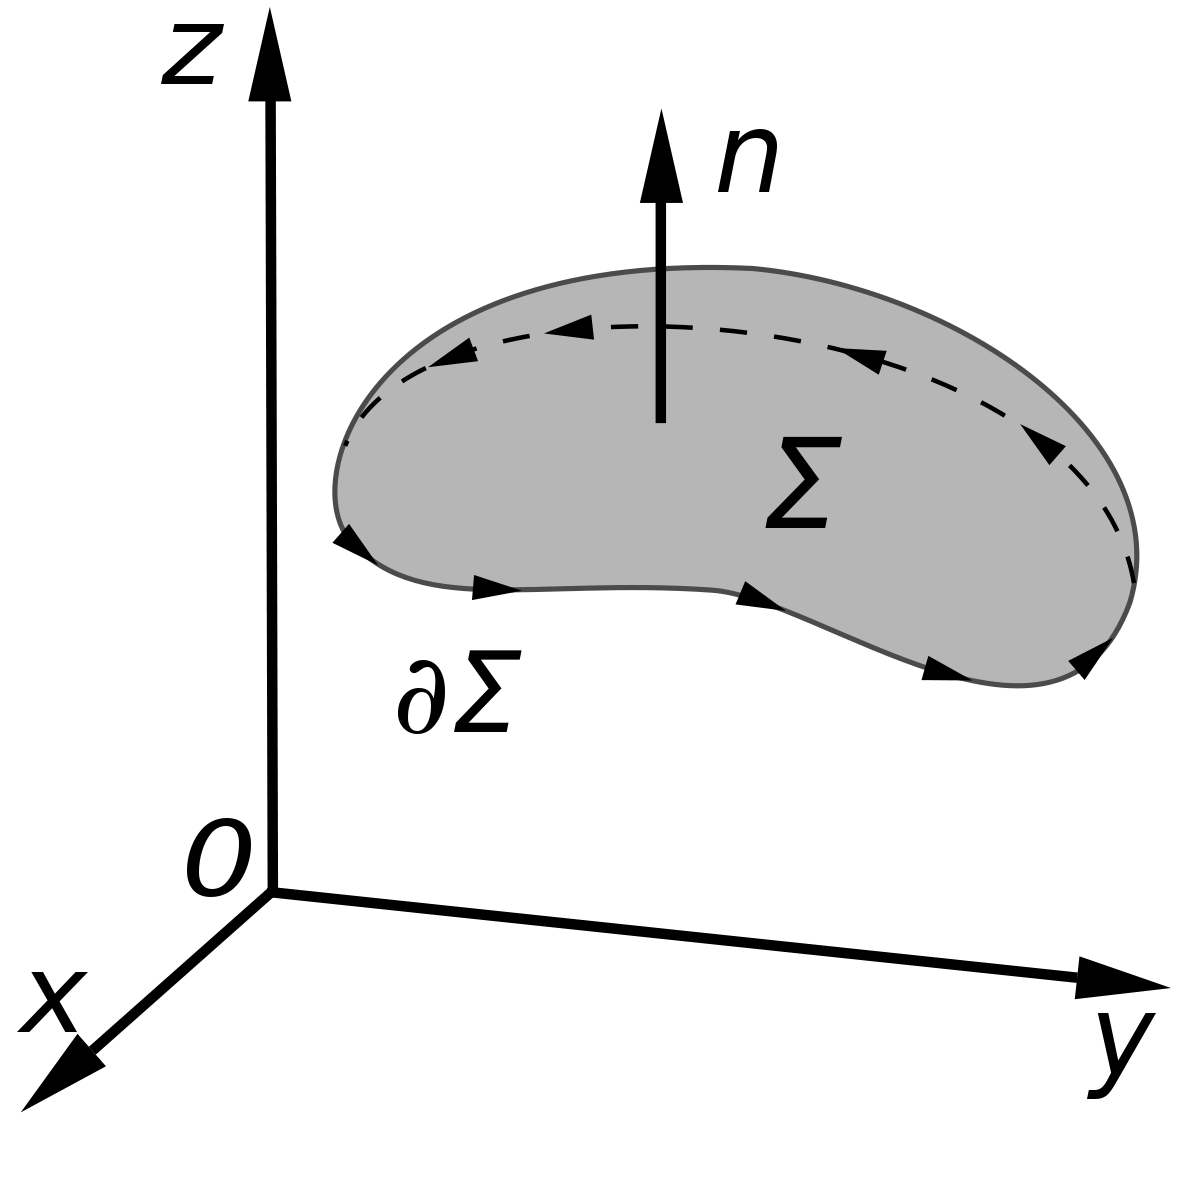
\includegraphics[width =0.5\textwidth]{1200px-Stokes'_Theorem.svg.png}
    \caption{A visual representation for the Stokes' theorem\cite{noauthor_stokes_2021}}
\end{figure}

\par\noindent\rule{\textwidth}{0.4pt}
\par\noindent\rule{\textwidth}{0.4pt}
\section{Electrostatics}
\subsection{The Holy Trinity}
\begin{align}
    &V = \frac{1}{4\pi\varepsilon_0}\int\frac{\rho}{\curly{r}}\dmr{\tau}\\[1em]
    %%
    &\laplacian V = -\frac{\rho}{\varepsilon_0}\\[1em]
    %%
    &E = - \nabla V\\[1em]
    %%
    &V = -\int \vec{E}\cdot \dmr{\vec{l}}\\[1em]
    %%
    &\vec{E} = \frac{1}{4\pi\varepsilon_0}\int \frac{\hat{\curly{r}}}{\curly{r}^2}\rho\dmr{\tau}\\[1em]
    %%
    &\nabla \cdot E = \frac{\rho}{\varepsilon_0}; \;\;\; \nabla \cross E = 0
\end{align}
\begin{figure}[h]
    \centering
    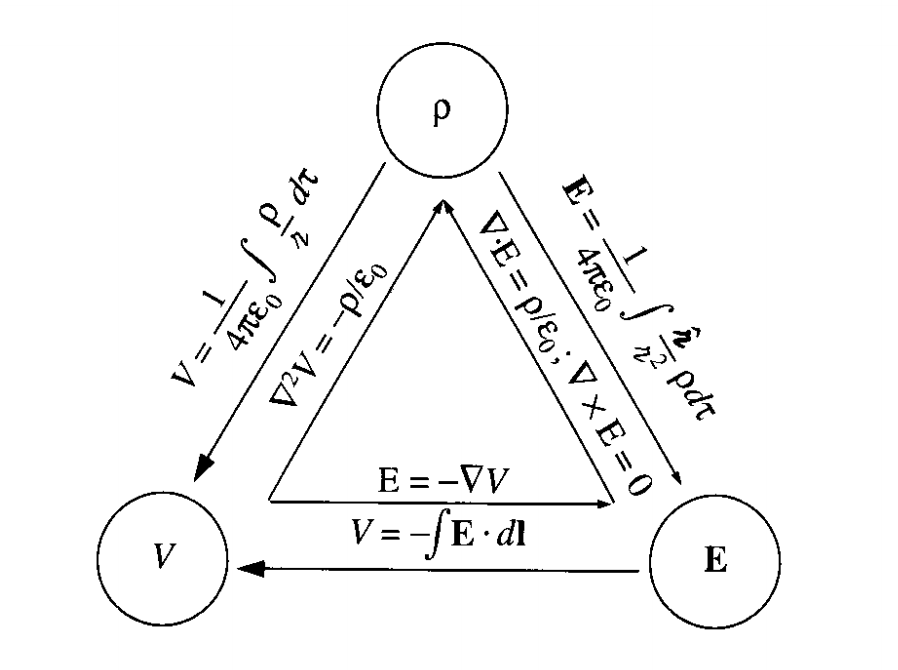
\includegraphics[width =0.5\textwidth]{holytrinity.png}
    \caption{The Griffith's holy trinity of electrostat\cite{Griffiths:611579}}
\end{figure}

\par\noindent\rule{\textwidth}{0.4pt}
\subsection{Electrostatic Boundary Conditions}
\begin{align}
    \hat{n}_2 \cdot [\vec{E}_1-\vec{E}_2] &= \frac{\sigma}{\varepsilon_0}\\[0.5em]
    \hat{n}_2 \cross [\vec{E}_1-\vec{E}_2] &= 0\\[0.5em]
    V_1 - V_2 &= 0
\end{align}
Note that here the "1" and "2" just refer to the different sides of the interface.

\par\noindent\rule{\textwidth}{0.4pt}













%%%%%%%%%%%%%%%%%%%%%%%%%%%%%%%%%%%%%%%%%%%%%%%%%%%%%%%%%%%%%%%%%
\newpage
\section*{References}
\addcontentsline{toc}{section}{\protect\numberline{}References}%
\printbibliography[heading = none]
%%%%%%%%%%%%%%%%%%%%%%%%%%%%%%%%%%%%%%%%%%%%%%%%%%%%%%%%%%%%%%%%%%
\end{document}